\section{AppConnector Example}
This section focuses on the AppConnector example program, including how to build it and what it does.
\subsection{Building}
Instructions for building the project for Linux and Windows follow.
\subsubsection{Linux}
Qt4 uses a function called qmake to automatically generate the Makefile for the project. It reads from a file with the .pro extension, and creates a Makefile based on the contents of the .pro file (see the Qt documentation for qmake for additional info). To create the Makefile, just type \texttt{qmake} in the AppConnectorExample folder (not the AppConnectorExample/src folder). Once this done, type \texttt{make}, and the project will be built. The executable is placed in the \texttt{AppConnectorExampole/bin} directory, and is called AppConnectorExample. To run it, cd to the bin directory, and type \texttt{./AppConnectorExample}. It should start and run.
\subsubsection{Windows}
To enter the Qt4 development environment, go to the Start Menu, select Qt4, and open the Qt4 Development command prompt. cd to the directory containing the AppConnectorExample. As in linux, the \texttt{qmake} function generates the approprate Makefile for the project, so do this now. When this is complete, you use the mingw make command to build the project. On Windows, you have the option of building a debug or release version. For now, do the release, because getting the debuggable version of Qt4 working can be difficult. To make the project, type \texttt{mingw32-make debug} in the AppConnectorExample folder. The executable is placed in the release/bin folder.

\subsubsection{OS X}
Someone who has tried Qt4 on a Max will have to let me know how well this works. I assume it is very similar to Linux/Unix.

\subsection{Running}
 \begin{figure}
\begin{center}
 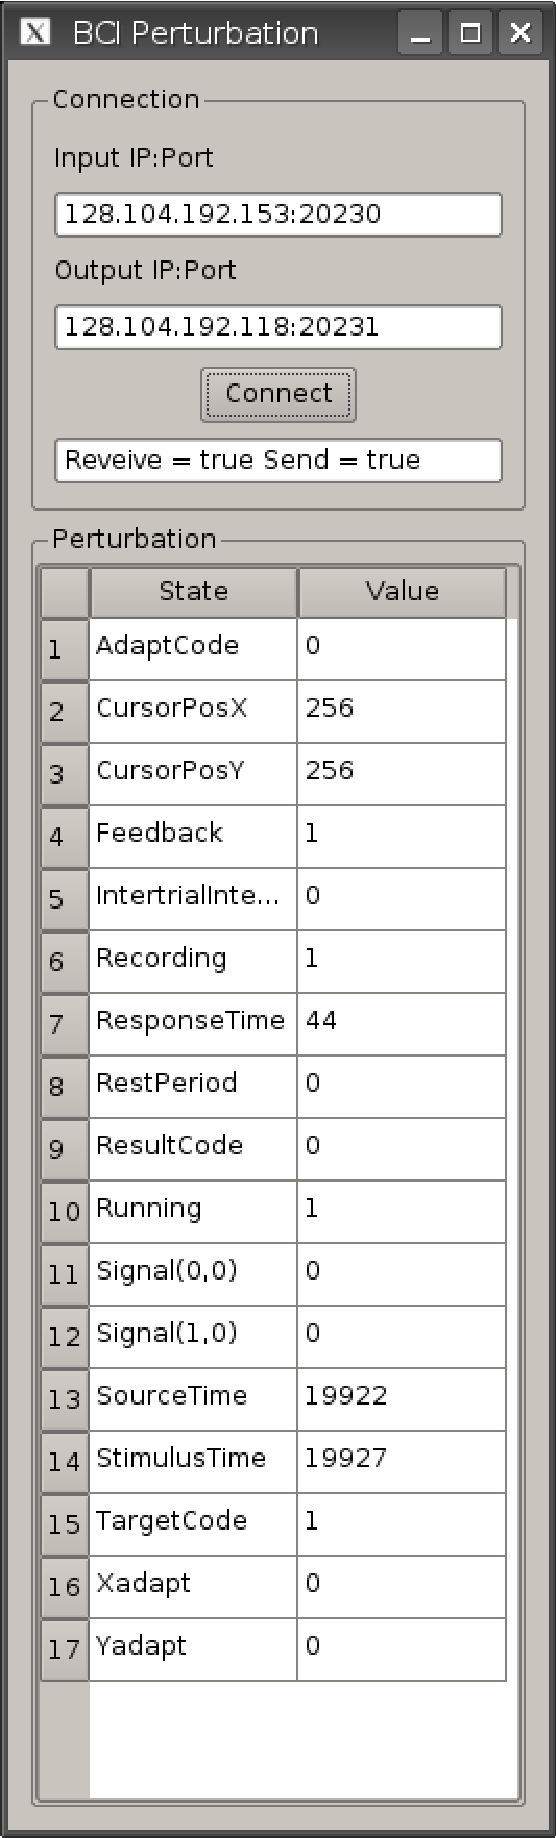
\includegraphics[scale=0.5]{appconnect}
\end{center}

\caption{AppConnectorExample}
\end{figure} 

After the project is built, run the program, and setup the connections as in Section \ref{sec:appdev} and Table \ref{tab:connect}. Once BCI2000 is running locally or remotely, press the Connect button to connect to BCI2000 on the addresses specified. If it works, the status box under the button will read ``Receive = true  Send = true'' If there is an error, one or both will read false.\\
When BCI2000 is in a suspended state, it is not writing any data to the UDP socket, so the program does not read them. When you press Start, BCI2000 begins writing the states to the socket, and the AppConnectorExample program will start reading them. The state names and values are displayed in the table at the bottom, and are updated every 100 ms.\\
To change a value, double-click the value column of the state you want to modify. A dialog box appears asking for the new value. Enter the value, and press Ok. The new value is written to BCI2000. For example, to stop the run, you can set the state Running to 0.